\documentclass[aspectratio=169]{beamer}
\usepackage[utf8]{inputenc}

\setbeamersize{text margin left=3mm,text margin right=3mm} 

\usetheme{Oxygen}
\usepackage{graphicx}
\usepackage{hyperref}
%\usepackage{movie15}
\usepackage{textpos}
\usepackage{fancybox}
\usepackage{colortbl}
\usepackage{rotating}
\usepackage{pgfplots}
% \usepackage{subfigure}
%\usepackage{subcaption}
\usepackage{multicol}
\usepackage{multirow}
\usepackage{amsmath,amssymb,amsfonts,amsbsy,dsfont}
\usepackage{mathrsfs}
\usepackage{amsthm}
\usepackage{bm}
\usepackage{array}
%\usepackage[caption=false]{subfig}
\usepackage{arydshln}
\usepackage{breakcites}
\usepackage{booktabs}
\usepackage{tabularx}
\usepackage{makecell}
\usepackage{amsmath}
\usepackage{tikz}
\usepackage{pgf-pie}
\usepackage{epsfig,epic,eepic,threeparttable,amscd,here,lscape,tabularx,graphicx }
\usepackage{booktabs}
\usepackage{tabu,array}
\usepackage{overpic}
\usepackage{microtype}

\usepackage{subcaption}
\usetikzlibrary{decorations.pathreplacing}


\let\oldcite\cite % store the original \cite command
\renewcommand{\cite}[1]{{\tiny\oldcite{#1}}}

\usepackage{bm}

\usepackage{etoolbox}

\DeclareUnicodeCharacter{2212}{-}


\usepackage[nopar]{lipsum} 

\newif\ifcomment
\newcommand{\Com}{\par\footnotesize\itshape\commenttrue}

\newenvironment{Itemize}
 {%
  \edef\Itemizecurrent{\the\font}%
  \itemize
  \preto{\item}{\ifcomment\par\Itemizecurrent\fi}%
 }{%
  \enditemize
 }


\title[]{Regularized Gaussian Functional Connectivity Network with Post-Hoc Interpretation for Improved EEG-based Motor Imagery-BCI Classification}
\vskip -0.7cm
\author{\normalsize{Daniel Guillermo Garc\'ia Murillo}\\ \scriptsize{dggarciam@unal.edu.co
}}
\institute{\includegraphics[width=0.15\textwidth]{../Tesis_document/Figures/EscudoUN2016.jpg}\\\scriptsize{
Universidad Nacional de Colombia \\ Signal Processing and Recognition Group - SPRG
\\
Advisor: Andrés Marino Álvarez-Meza, Ph.D.\\
Co-advisor: César Germán Castellanos-Domíguez, Ph.D.\\
\vspace{-0.3cm}
}}

% \date[]{\scriptsize{Signal Processing and Recognition Group - SPRG\\
% Department of Electrical, Electronic and Computer Engineering\\
% Universidad Nacional de Colombia - Sede Manizales\\
% 2024}}
\date[]{\scriptsize{\today}}



\setbeamercovered{dynamic}
\setbeamertemplate{navigation symbols}{}

\begin{document}

{\setbeamertemplate{headline}{}
\setbeamertemplate{footline}{}
\begin{frame}{}
\vspace{-0.7cm}
    \titlepage 
\end{frame}
}


\newif\iflattersubsect

% \AtBeginSection[] {
%     \begin{frame}
%     \frametitle{Outline} %
%     \tableofcontents[currentsection, sections={1-6}]  
%     \end{frame}
%     \lattersubsectfalse
% }

% \AtBeginSection[] {
%     \begin{frame}
%     \frametitle{Outline I} %
%     \tableofcontents[currentsection, sections={1-6}]  
%     \end{frame}
%     \only<7-9>{
%         \begin{frame}
%         \frametitle{Outline II} %
%         \tableofcontents[currentsection, sections={7-9}]  
%         \end{frame}
%     }
%     \lattersubsectfalse
% }

\AtBeginSection[] {
    \ifnum\thesection<7
        \begin{frame}
        \frametitle{Outline I} %
        \tableofcontents[currentsection, sections={1-6}]  
        \end{frame}
    \else
        \begin{frame}
        \frametitle{Outline II} %
        \tableofcontents[currentsection, sections={7-9}]  
        \end{frame}
    \fi
    \lattersubsectfalse
}

\AtBeginSubsection[] {
    \ifnum\thesection<7
        \begin{frame}
        \frametitle{Outline I} %
        \tableofcontents[currentsubsection, sections={1-6}]  
        \end{frame}
    \else
        \begin{frame}
        \frametitle{Outline II} %
        \tableofcontents[currentsubsection, sections={7-9}]  
        \end{frame}
    \fi
    \lattersubsectfalse
}

\section[Motivation]{Motivation}

\begin{frame}{Brain computer interface (BCI)}
    \centering
    BCI provide people external world communication by translating brain signals~\cite{khan2020review}
    \begin{figure}[!ht]
        \centering
        \resizebox{0.8\linewidth}{!}{\includegraphics{figures/Motivation_BCI.png}}
        % \caption{Functional connectivity estimators classified based on direct or indirect, time or frequency domain and linear or nonlinear. The varying shades of orange represent different sensitivities to volume conduction.}
    \end{figure}

\end{frame}

\begin{frame}{Brain computer interface (BCI)}
    \begin{columns}
        \column{0.6\textwidth}
        \begin{figure}
            \centering
            \resizebox{0.7\linewidth}{!}{\includegraphics{figures/pie_bci}}
            % \includegraphics[width=0.7\linewidth]{figures/BCI_applications.png}
            % \caption{Distribution of BCI Applications~\footnotemark[1].}
        \end{figure}
        \column{0.4\textwidth}
            \begin{itemize}
                \item Over 150 companies specializing in BCI as of 2019.
                \item BCI market valued at $228$ million in 2019, projected to reach $460$ million by 2029~\footnotemark[2].
            \end{itemize}
    \end{columns}
    \footnotetext[1]{\textbf{{Image}:} {Adapted from} \href{https://www.weforum.org/agenda/2024/06/the-brain-computer-interface-market-is-growing-but-what-are-the-risks/}{The World Economic Forum 2024}}
    \footnotetext[2]{\href{https://www.marketreportsworld.com/enquiry/request-sample/23789843}{Global Brain Computer Interface Market Research Report 2023}}
\end{frame}


\begin{frame}{Motor Imagery (MI)}
    \centering
    MI is a widely studied BCI paradigm that allows external motor communication~\cite{cattan2018recommendations}.
    \vspace{3em}
    \begin{columns}
        \column{0.5\textwidth}
        \centering
        \includegraphics[width=0.7\linewidth]{figures/Motor_imagery.png}
        \column{0.5\textwidth}
            \textbf{Applications:}
            \begin{itemize}
                \item Recovery of motor functionality \cite{bonci2021introductory}.
                \item Motor rehabilitation \cite{sitaram2017closed}.
                \item Virtual reality  \cite{cattan2018recommendations}.
                \item Gaming \cite{ahn2014review}.
                \item Skill acquisition \cite{casimo2017bci}.
            \end{itemize}
    \end{columns}
\end{frame}

\begin{frame}{Neuroimaging techniques}
    \begin{columns}
        \column{0.3\textwidth}
            \begin{itemize}
                \item MI involves fast-evolving cognitive processes \cite{varbu2022past}
                \item EEG and MEG have remarkable temporal precision \cite{alsharif2020neuromarketing}
                \item EEG is portabile and cost-effective \cite{janapati2023advances, hosseini2020review}
            \end{itemize}
        \column{0.7\textwidth}
            \begin{figure}[h!]
                \centering
                \resizebox{1\linewidth}{!}{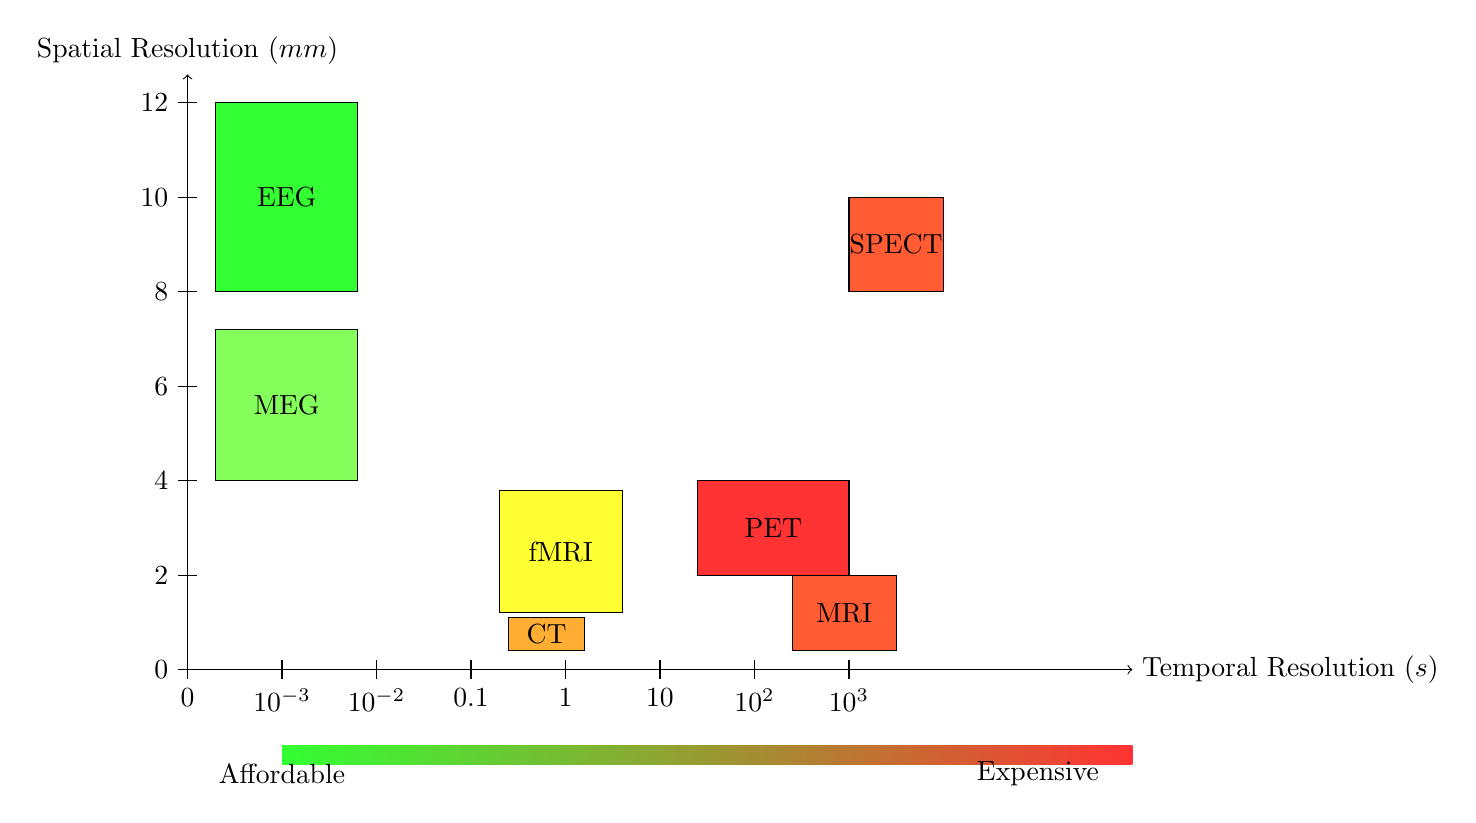
\begin{tikzpicture}[scale=1.2]

% Draw axes
% EEG 0.2
% MEG 0.4
% fMRI 0.8
% CT 0.6
% MRI 0.7
% PET 0.9
% SPECT 0.8

\definecolor{eegcolor}{HTML}{00FF00}
\definecolor{megcolor}{HTML}{66FF33}
\definecolor{fmricolor}{HTML}{FFFF00}
\definecolor{ctcolor}{HTML}{FF9900}
\definecolor{mricolor}{HTML}{FF3300}
\definecolor{petcolor}{HTML}{FF0000}
\definecolor{spectcolor}{HTML}{FF3300}
% X-axis labels
\draw[->] (0,0) -- (10,0) node[right] {Temporal Resolution $(s)$};
\draw (0,0.1) -- (0,-0.1) node[below] {$0$};
\draw (1,0.1) -- (1,-0.1) node[below] {$10^{-3}$};
\draw (2,0.1) -- (2,-0.1) node[below] {$10^{-2}$};
\draw (3,0.1) -- (3,-0.1) node[below] {$0.1$};
\draw (4,0.1) -- (4,-0.1) node[below] {$1$};
\draw (5,0.1) -- (5,-0.1) node[below] {$10$};
\draw (6,0.1) -- (6,-0.1) node[below] {$10^2$};
\draw (7,0.1) -- (7,-0.1) node[below] {$10^3$};

% Y-axis labels
\draw[->] (0,0) -- (0,6.3) node[above] {Spatial Resolution $(mm)$};
\draw (0.1,0) -- (-0.1,0) node[left] {$0$};
\draw (0.1,1) -- (-0.1,1) node[left] {$2$};
\draw (0.1,2) -- (-0.1,2) node[left] {$4$};
\draw (0.1,3) -- (-0.1,3) node[left] {$6$};
\draw (0.1,4) -- (-0.1,4) node[left] {$8$};
\draw (0.1,5) -- (-0.1,5) node[left] {$10$};
\draw (0.1,6) -- (-0.1,6) node[left] {$12$};

\fill[left color=eegcolor!80, right color=petcolor!80] (1,-1) rectangle ++(9,0.2);

\draw (9,-1.1) node[align=center] {Expensive};
\draw (1,-1.1) node[align=center] {Affordable};

% EEG (x,y)
\draw[fill=eegcolor!80] (0.3,4) rectangle (1.8,6) node[pos=.5] {EEG};

% MEG
\draw[fill=megcolor!80] (0.3,2) rectangle (1.8,3.6) node[pos=.5] {MEG};

% fMRI
\draw[fill=fmricolor!80] (3.3,0.6) rectangle (4.6,1.9) node[pos=.5] {fMRI};

% CT
\draw[fill=ctcolor!80] (3.4,0.2) rectangle (4.2,0.55) node[pos=.5] {CT};

% MRI
\draw[fill=mricolor!80] (6.4,0.2) rectangle (7.5,1) node[pos=.5] {MRI};

% PET
\draw[fill=petcolor!80] (5.4,1) rectangle (7,2) node[pos=.5] {PET};

% SPECT
\draw[fill=spectcolor!80] (7,4) rectangle (8,5) node[pos=.5] {SPECT};

\end{tikzpicture}}
                % \caption{Comparison of neuroimaging techniques: spatial and temporal resolutions, and relative costs}\label{fig:neuroimagig}
            \end{figure}
    \end{columns}
\end{frame}

\begin{frame}{Experimental setup for MI-based BCIs}
    \begin{columns}
        \column{0.6\textwidth}
            \begin{figure}[!ht]
                \centering
                \includegraphics[width=0.8\linewidth]{../Tesis_document/Figures/preliminaries/EEG-setup.png}
                % \caption{Experimental setup for MI-based BCIs. \textbf{{Source}
                %         :} {Adapted from} \cite{grigorev2021bci}}
            \end{figure}
        \column{0.4\textwidth}
            \begin{itemize}
                \item EEG headsets are equipped with $1$ to $256$ electrodes \cite{grigorev2021bci}.
                \item Visual cues are often used to guide MI tasks during EEG recordings \cite{hosseini2020review}.
            \end{itemize}
    \end{columns}
    \footnotetext[1]{\textbf{{Image}:} {Adapted from} \cite{grigorev2021bci}}
\end{frame}


\begin{frame}{Sensorimotor rhythms (SMRs)}
    \begin{columns}
        \column{0.4\textwidth}
            \begin{itemize}
                \item EEG signals contains multiple electrical variations (rhythms) \cite{barios2019synchronization}.
                \item Sensorimotor Rhythms (SMRs) occur in the brain's sensorimotor cortex \cite{altaheri2023deep}. 
                \item SMRs contain spectral-spatio-temporal patterns of MI tasks \cite{li2019motor}.
            \end{itemize}
        \column{0.6\textwidth}
            \begin{figure}[!ht]
                \centering
                \includegraphics[width=0.7\linewidth]{figures/SM_area.png}
            \end{figure}
    \end{columns}
    \footnotetext[1]{\textbf{{Image}:} {Adapted from} \cite{bookbiology20001}}
\end{frame} 


\begin{frame}{MI-EEG feature extraction}
    \begin{columns}
        \column{0.7\textwidth}
            \begin{figure}[!ht]
                \centering
                \includegraphics[width=0.7\linewidth,trim={0 0 0 10},clip]{figures/RAW_EEG.png}
                % \caption{Raw EEG signal representation}
            \end{figure}
        \column{0.3\textwidth}
            \begin{itemize}
                \item High number of channels and sampling rate \cite{chevallier2024largest}.
                \item Huge number of data points \cite{singh2021comprehensive}.
                \item Feature extraction strategies are required to reduce dimentionality \cite{ai2019feature}.
            \end{itemize}
    \end{columns}
    \centering
    
\end{frame}

\begin{frame}{Single channel feature extraction}
    \begin{columns}
        \column{0.4\textwidth}
            \begin{itemize}
                \item Capture rhythms on specific EEG channels \cite{samuel2017towards}.
                \item Time domain: statistical \cite{hamedi2014neural}, Hjorth \cite{yilmaz2018quasi}, etc.
                \item Spetral doamin: Power spectral density \cite{oikonomou2017comparison}, Welch's periodigram \cite{roy2022comparative}, spectral entropy \cite{sarraf2017eeg}, etc.
            \end{itemize}
        \column{0.6\textwidth}
            \begin{figure}[!ht]
                \centering
                \includegraphics[width=0.6\linewidth,trim={0 110 40 40},clip]{figures/Cxsbj1gaussacc86.85-eps-converted-to.pdf}
                % \caption{Brain area activation when performing motor imagery tasks}
            \end{figure}
    \end{columns}
    \vspace{3em}
    \centering
    Executing or imagining motor tasks activates multiple brain areas, patterns that single-channel features fail to capture \cite{chiarion2023connectivity}.
\end{frame}


\begin{frame}{Multi channel feature extraction}
    \begin{columns}
        \column{0.5\textwidth}
            \begin{figure}[!ht]
                \centering
                \includegraphics[width=1\linewidth]{figures/connectivities.png}
                % \caption{Three  types of brain connectivity: structural, effective, and functional, each describing interactions between brain regions \cite{ismail2020graph}.}
            \end{figure}
        \column{0.5\textwidth}
            \begin{itemize}
                \item Structural connectivity (SC) focuses on physical connections, fails to capture short-living events \cite{thiebaut2020brain}
                \item Effective connectivity (EC) describes direct connections and requires deep cognitive process understanding to select the best causal model \cite{chiarion2023connectivity}.
                \item Functional connectivity (FC) can describe directed or non-directed connectives usually via statistical correlation \cite{cao2022brain}
            \end{itemize}
    \end{columns}
    \vspace{3em}
    \centering
    FC's simplicity, low computational demands, and lack of rigid assumptions make it ideal for MI-BCI applications \cite{he2019electrophysiological}.
\end{frame}

\begin{frame}{Signal Processing and Recognition Group - SPRG}
    The SPRG has been working on the design of ML and DL models to improve the performance and explainability of EEG-based MI-BCIs \cite{collazos2023posthoc}.
    \centering
    \includegraphics[width=0.7\linewidth]{figures/bcisoft.jpeg}
\end{frame}

\section{Problem statement}

\begin{frame}{Problem statement}
    \begin{figure}[!ht]
        \centering
        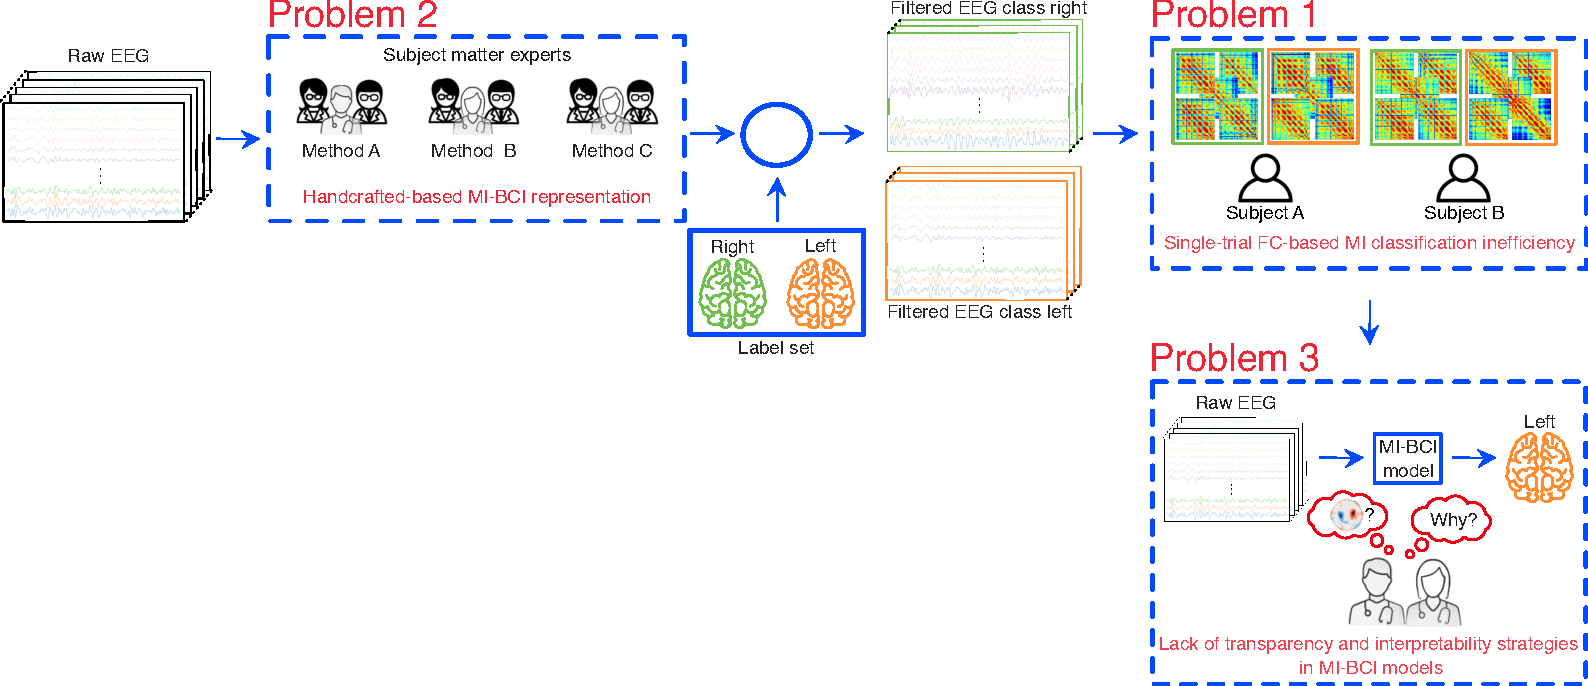
\includegraphics[width=1\linewidth]{../Tesis_document/Figures/problem_statement/general_problem.pdf}
        % \caption{Illustration of the three key challenges in FC EEG-based MI-BCI: noise and variability in single
        % trial FC estimators, handcrafted-based subject-specific EEG-based MI-BCI Representation, and the need for
        % model transparency}
    \end{figure}
\end{frame}

\begin{frame}{Single-Trial FC MI Classification Inefficiency}
    \begin{figure}[!ht]
        \centering
        \includegraphics[width=1\linewidth]{../Tesis_document/Figures/problem_statement/problem1_FV.pdf}
        % \caption{Single-trial FC-based MI classification inefficiency graphical scheme.}
    \end{figure}
\end{frame}

\begin{frame}{Handcrafted-based Subject-Specific EEG-based MI-BCI Representation}
    \begin{figure}[!ht]
        \centering
        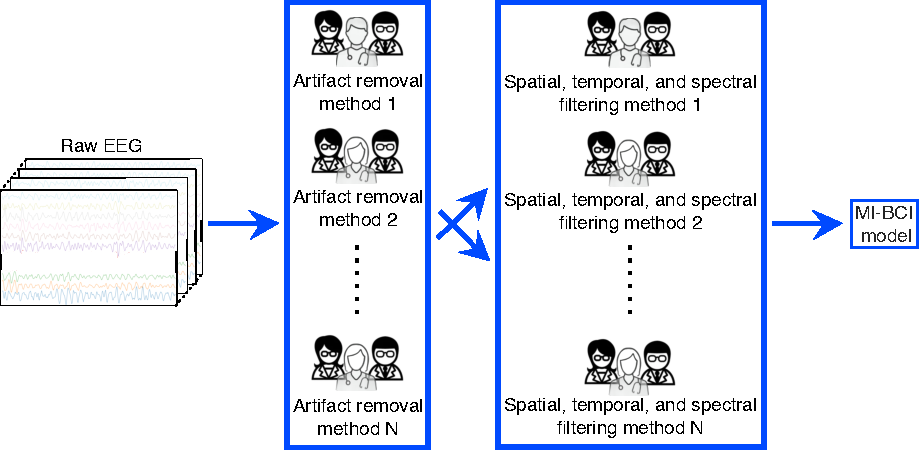
\includegraphics[width=0.9\linewidth]{../Tesis_document/Figures/problem_statement/problem2_VF.pdf}
        % \caption{llustration of challenges in EEG signal representation, including strategies for artifact removal and implementing spatial, temporal, and frequency filters.}
    \end{figure}
\end{frame}


\begin{frame}{Lack of Transparency and Interpretability Strategies in MI-BCI}
    \begin{figure}[!ht]
        \centering
        \includegraphics[width=1\linewidth]{../Tesis_document/Figures/problem_statement/problem3_FV.pdf}
        % \caption{Transparency and interpretability challenges in MI-BCI models graphical scheme.}
    \end{figure}
\end{frame}


\begin{frame}{Research question}
\centering
How can a single-trail FC be developed to manage non-stationary EEG subject-specific representations, handle spurious connectivities, and encode non-linear spatial, temporal, and spectral discriminative and interpretable MI patterns?
\end{frame}

\section{State of the art}
\subsection{Single-Trial FC in MI-BCI}

\begin{frame}{Functional Connectivity Estimators}
    \begin{figure}[!ht]
        \centering
        \resizebox{0.7\linewidth}{!}{\includegraphics{../Tesis_document/Figures/state_of_art/sota1_EFC.pdf}}
        % \caption{Functional connectivity estimators classified based on direct or indirect, time or frequency domain and linear or nonlinear. The varying shades of orange represent different sensitivities to volume conduction.}
        % Abbreviations: Corr, correlation \cite{fagerholm2020dynamic}; MSC, magnitude square coherence \cite{cattai2021phase}; IPC, imaginary part of the coherence  \cite{cao2022brain}; PC, partial coherence \cite{gonzalez2020network}; PLI, phase lag index  \cite{siviero2023functional}; WPLI, weighted phase lag index \cite{gonzalez2020network}; PLV, phase locking value \cite{cattai2021phase}; MI, mutual information \cite{gu2023decoding}; SL, synchronization likelihood \cite{gonzalez2021network}; Cross-corr, cross-correlation \cite{roy2022comparative}; GC, Granger causality \cite{rezaei2023classification}; TE, transfer entropy \cite{rezaei2023classification}; DTF, directed transfer function \cite{rezaei2023classification}; PDC, partial directed coherence\cite{gaxiola2017using}}
    \end{figure}
\end{frame}


\begin{frame}{Feature Extraction from FC}
    \begin{figure}[!ht]
        \centering
        \resizebox{0.95\linewidth}{!}{\includegraphics{../Tesis_document/Figures/state_of_art/sota1_FE.pdf}}
        % \caption{Functional connectivity estimators classified based on direct or indirect, time or frequency domain and linear or nonlinear. The varying shades of orange represent different sensitivities to volume conduction.}
    \end{figure}
\end{frame}


\subsection{Subject-Specific EEG Representation for MI-BCI}


\begin{frame}{Input Formulation in Deep Learning}
    \begin{figure}[!ht]
        \centering
        \resizebox{0.85\linewidth}{!}{\includegraphics{../Tesis_document/Figures/state_of_art/sota2_input_v2.pdf}}
        % \caption{Functional connectivity estimators classified based on direct or indirect, time or frequency domain and linear or nonlinear. The varying shades of orange represent different sensitivities to volume conduction.}
    \end{figure}
\end{frame}


\begin{frame}{Deep Learning Architectures}
    \begin{figure}[!ht]
        \centering
        \resizebox{0.85\linewidth}{!}{\includegraphics{../Tesis_document/Figures/state_of_art/sota2_DLAV2.pdf}}
        % \caption{Functional connectivity estimators classified based on direct or indirect, time or frequency domain and linear or nonlinear. The varying shades of orange represent different sensitivities to volume conduction.}
    \end{figure}
\end{frame}

\subsection{Interpretability Strategies in MI-BCI}

\begin{frame}{Interpretability Strategies in MI-BCI}
    \begin{figure}[!ht]
        \centering
        \resizebox{0.9\linewidth}{!}{\includegraphics{../Tesis_document/Figures/state_of_art/sota3_methods.pdf}}
        % \caption{Functional connectivity estimators classified based on direct or indirect, time or frequency domain and linear or nonlinear. The varying shades of orange represent different sensitivities to volume conduction.}
    \end{figure}
\end{frame}

\section{Aims}

\begin{frame}{General Objective}
    To develop a single-trial indirect functional connectivity framework, accompanied by regularized deep learning approaches, to extract pertinent subject-specific non-linear spatio-temporal-frequency patterns from non-stationary EEG data, improving the MI-BCI system's accuracy and interpretability.
\end{frame}

\begin{frame}{Specific Objectives}
\centering
\begin{itemize}
    \setlength\itemsep{2em}
	\item[1] To develop a single-trial indirect FC for enhanced nonlinear feature extraction, preserving the spatio-temporal-frequency interpretability while favoring the classification performance in MI-BCI and avoiding spurious connectivities.
 
	\item[2] To extend the proposed single-trial FC within a deep learning scheme that handles artifacts and EEG representations, necessitating minimal preprocessing efforts from raw signals.
 
	\item[3] To develop a transparency and interpretability strategy dedicated to MI-BCI classification that emphasizes spatial-temporal-spectral pattern domains, incorporating a qualitative and quantitative relevance analysis assessment.
\end{itemize}
\end{frame}

\section{Outline and contributions}

\begin{frame}{Outline and contributions}
    \begin{figure}[h!]
        \centering
        \includegraphics[scale=0.65]{../Tesis_document/Figures/outline_and_contributions/general_contributions.pdf}
        % \caption{Schematic display of the main thesis contributions, including the single-trial FC estimator and feature extraction, an end-to-end approach from EEG representations to MI classification, and quantitative and qualitative strategies for model interpretation\label{fig:img_gen_outline}}
    \end{figure}
\end{frame}

\section{Datasets}

\begin{frame}{BCI Competition IV Dataset IIa - DBI MI}
    \textbf{One-day data collection}
    \begin{figure}[!h]
        \centering
        \includegraphics[width=\linewidth]{../Tesis_document/Figures/preliminaries/BCI2a_schema.pdf}
      \end{figure}
      \begin{columns}
        \column{0.5\textwidth}
            \centering
            \textbf{Acquisition protocol}
            \begin{figure}[!ht]
                \centering
                \resizebox{0.9\linewidth}{!}{\input{../Tesis_document/Figures/preliminaries/procedure_BCI2a.tikz}}
            \end{figure}
        \column{0.5\textwidth}
            \centering
            \textbf{Electrode montage}
            \begin{figure}[!ht]
                \centering
                \resizebox{0.8\linewidth}{!}{\includegraphics[width=0.6\linewidth]{../Tesis_document/Figures/preliminaries/bcielectrodes.PNG}}
            \end{figure}
    \end{columns}
\end{frame}

\begin{frame}{Gamma Motor Execution Database—DBII ME}
    b
\end{frame}

\begin{frame}{MI BCI EEG Giga Science Database - DBIII MI}
    c
\end{frame}

\section{Proposal and Results}

\subsection{Single-Trial Kernel-based Functional Connectivity for Enhanced Feature Extraction in EEG-based MI-BCI}

\begin{frame}{a}
    a
\end{frame}

\subsection{KCS-FCnet: Kernel Cross-Spectral Functional Connectivity Network for Automatic EEG Representation in MI-BCI}

\begin{frame}{a}
    a
\end{frame}

\subsection{IRKCS-FCnet: Interpretable Regularized Kernel Cross-Spectral Functional Connectivity Network with Qualitative and Quantitative Post-Hoc and Intrinsic Explainability}

\begin{frame}{a}
    a
\end{frame}

% Electrical variations can be used to describe cognitive states \cite{li2019brain}

\section{References}
% ------------------------------------------------------------------------
\begin{frame}[allowframebreaks]%,noframenumbering]
\frametitle{References}
{\tiny 
\bibliographystyle{apalike}
\bibliography{../Tesis_document/References}
}
\end{frame}

\end{document}